\documentclass[12pt, letterpaper, twoside]{book}
\raggedbottom
\usepackage{graphicx}
\graphicspath{ {images/} }
\usepackage[utf8]{inputenc}
\usepackage{fullpage}
\usepackage[paperheight=11in,paperwidth=8.5in,margin=0in]{geometry}
\usepackage{amsmath}
\usepackage{listings}
\date{27nd May 2021}
\begin{document}
\begin{titlepage}
	\begin{center}
       \vspace*{5cm}
       \bfseries\Large
    	Assignment 3\\
    	Of\\
    	Modelling \& Simulation Lab (CS1052)\\
        \vskip1cm
        Masters of Technology in Computer Science And Engineering\\
        \vskip1cm
        submitted by\\
    	Arghya Bandyopadhyay\\
    	RollNo. 20CS4103\\
    	\vskip1cm
    	submitted to\\
    	Dr Nanda Dulal Jana\\
    	Assistant Professor\\
    	Dept. of CSE\\
    	\vskip1cm
    	
\includegraphics[width=4cm]{NITDGP}\\
    	National Institute of Technology, Durgapur\\
    \end{center}
\end{titlepage}
\begin{center}
\textbf{\\Problem 1}
\end{center}
\begin{flushleft}
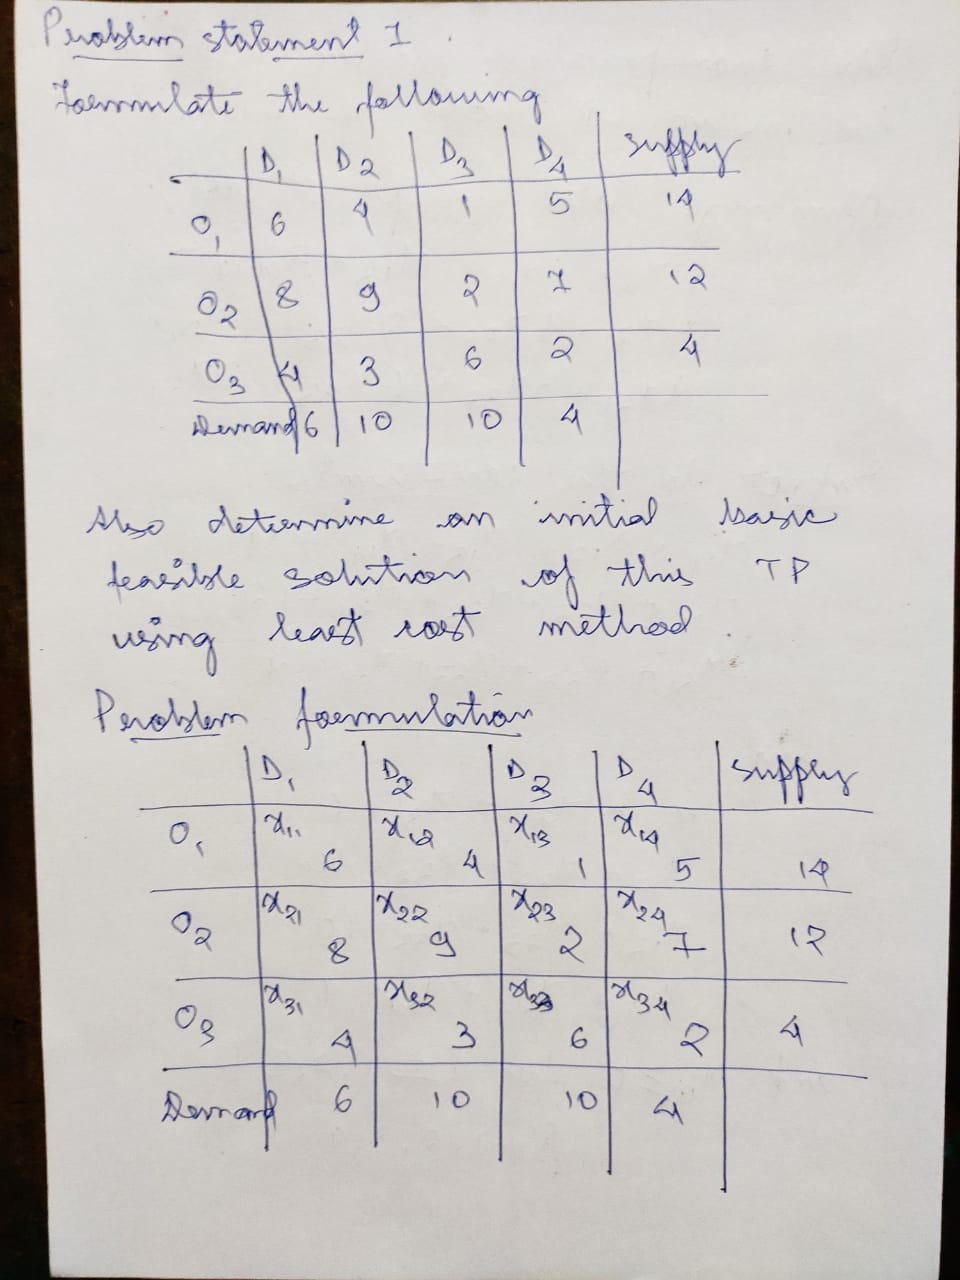
\includegraphics[width=\paperwidth, height=10in]{Page1}
\end{flushleft}
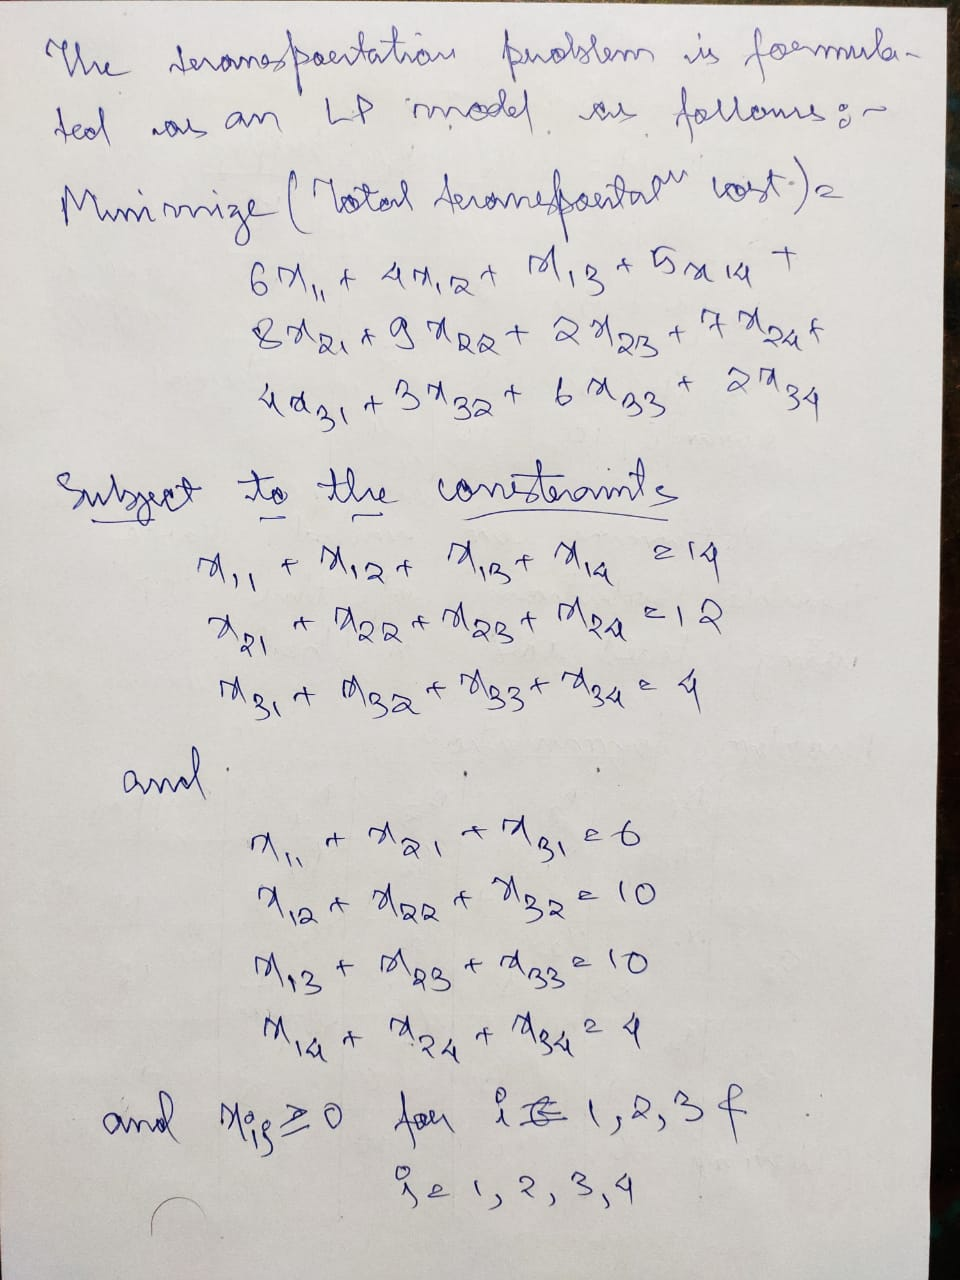
\includegraphics[width=\paperwidth, height=\paperheight]{Page2}
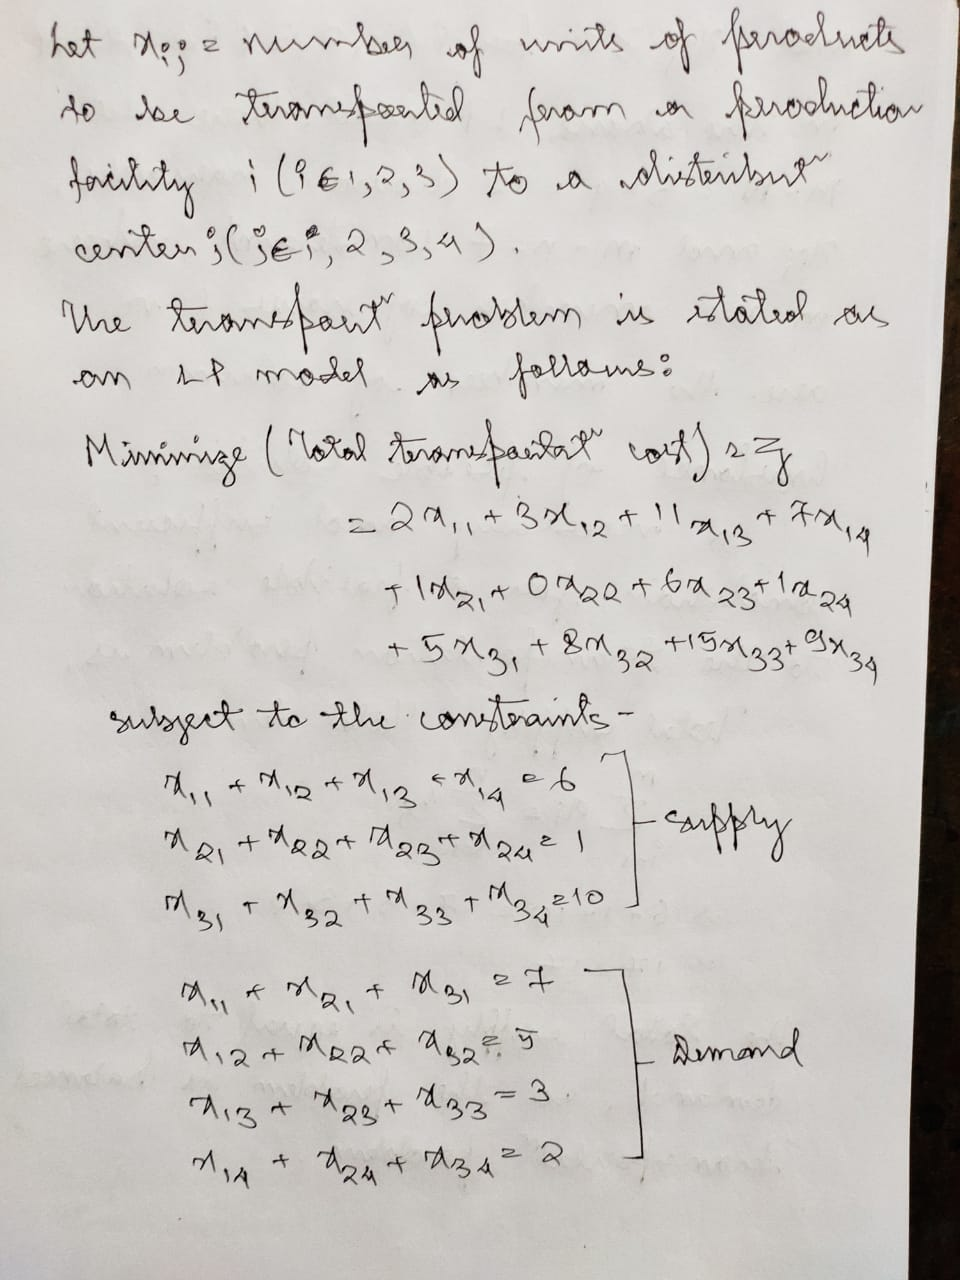
\includegraphics[width=\paperwidth, height=\paperheight]{Page3}
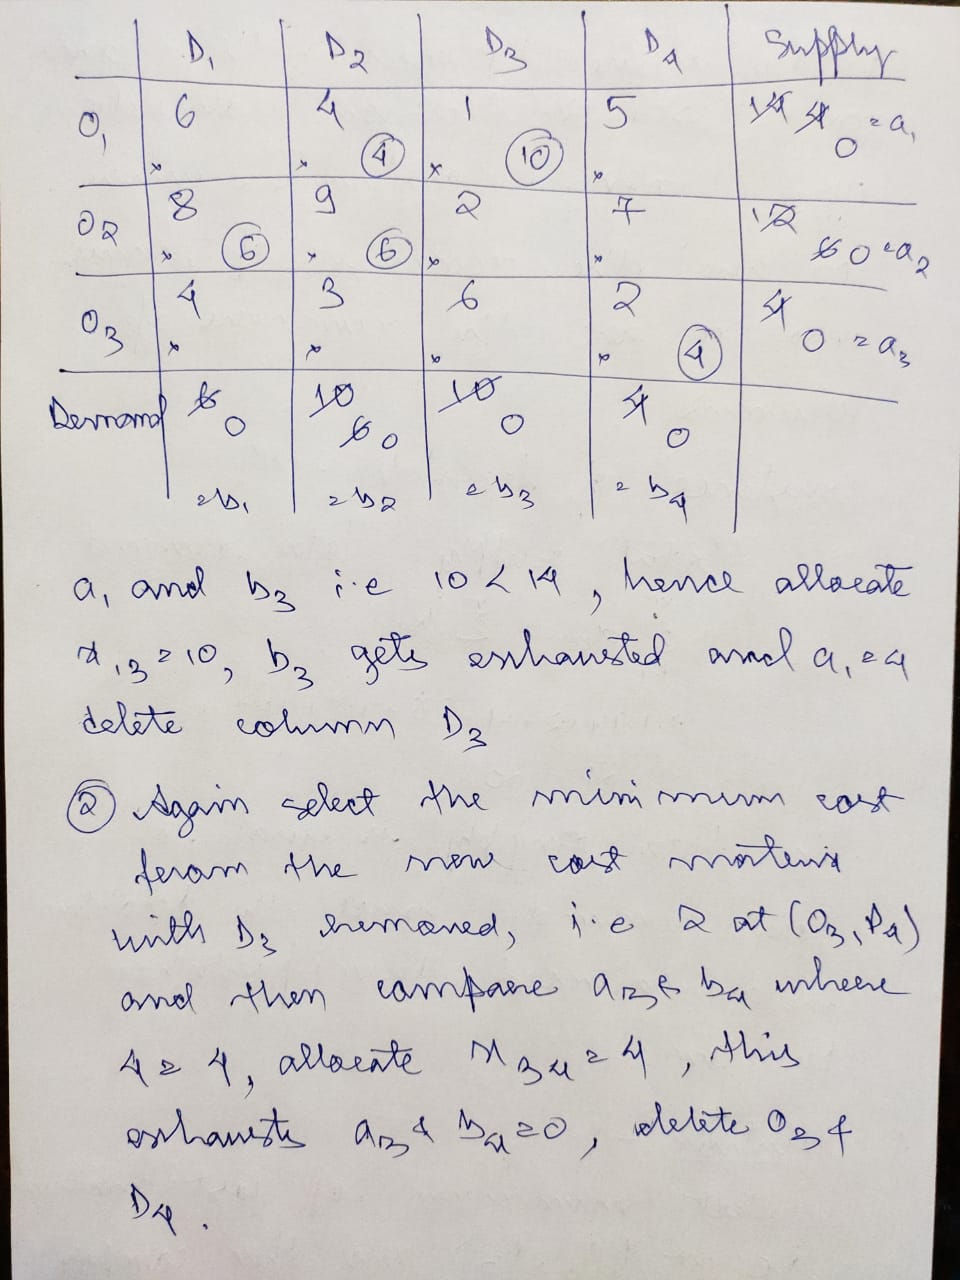
\includegraphics[width=\paperwidth, height=\paperheight]{Page4}
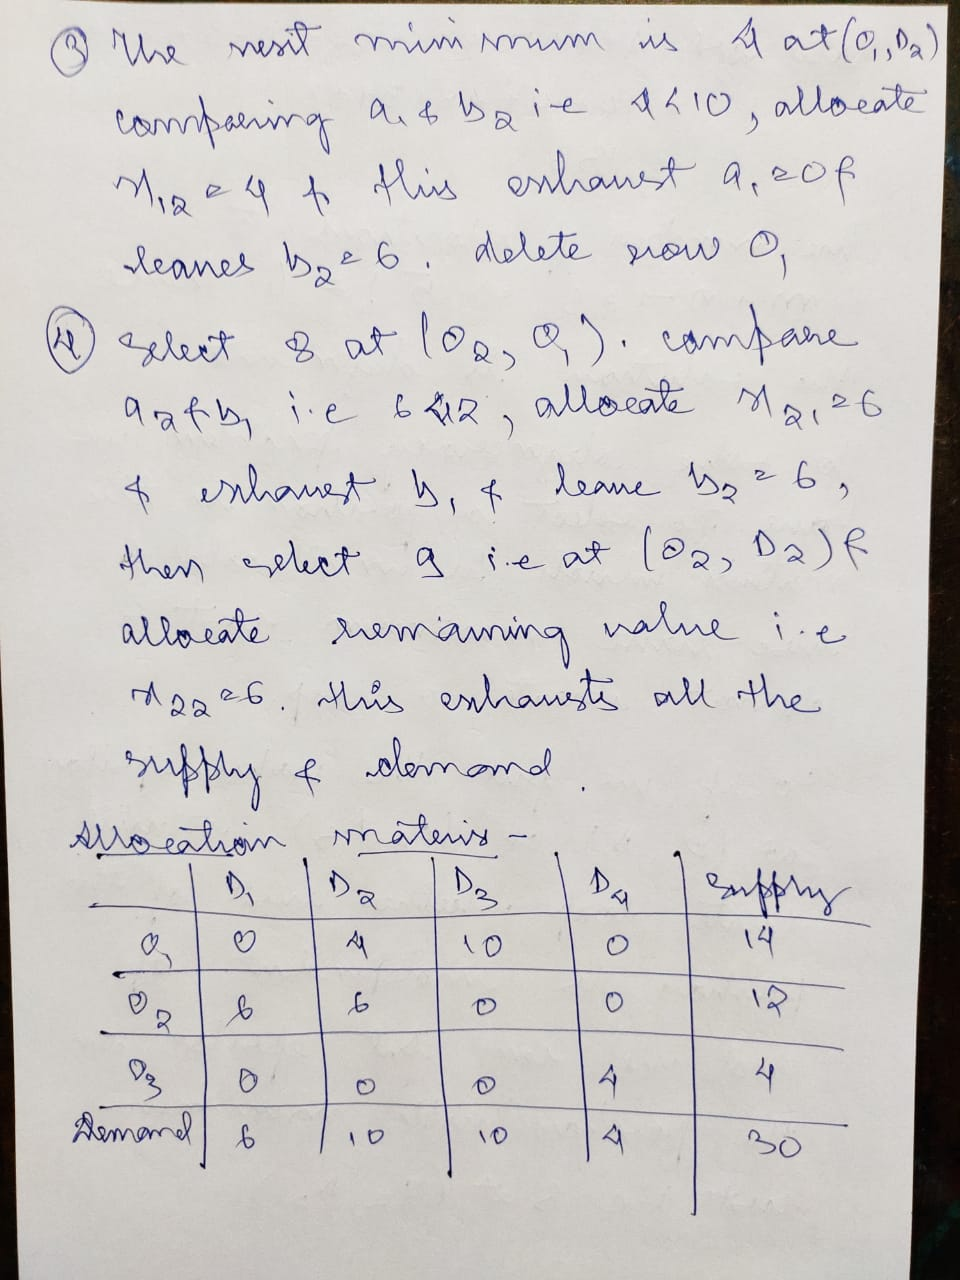
\includegraphics[width=\paperwidth, height=\paperheight]{Page5}
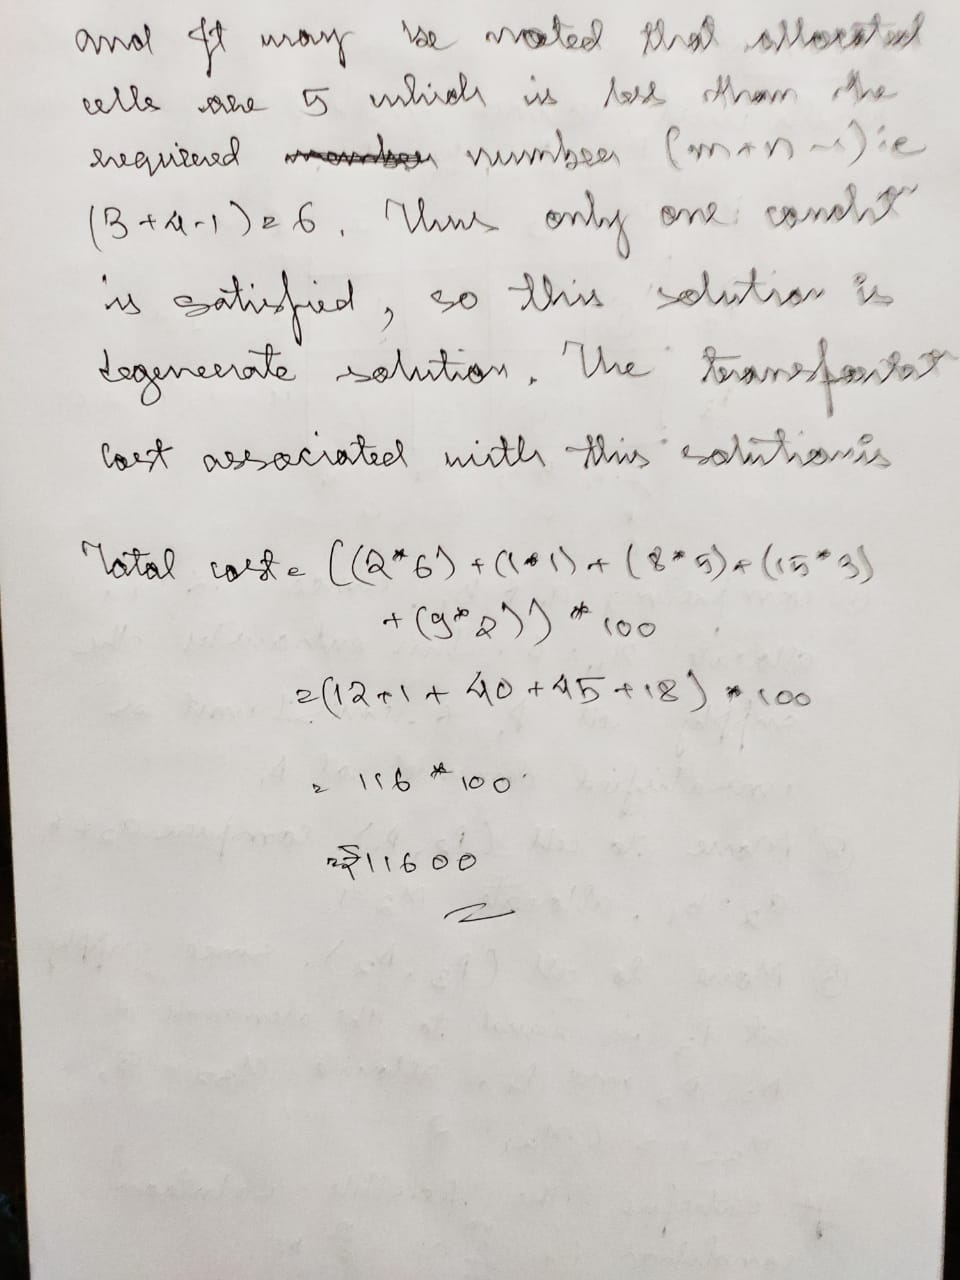
\includegraphics[width=\paperwidth, height=\paperheight]{Page6}
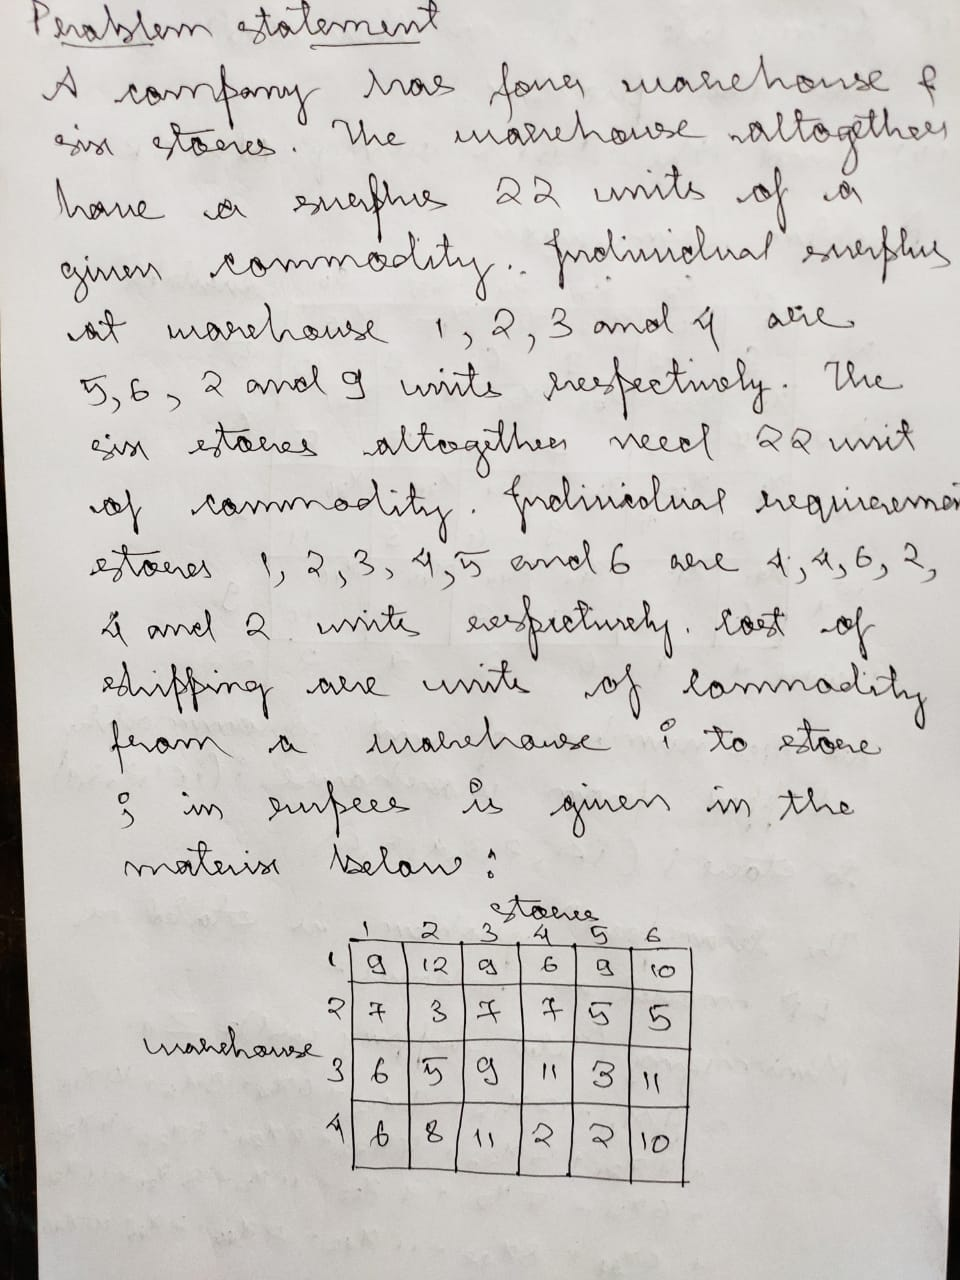
\includegraphics[width=\paperwidth, height=\paperheight]{Page7}
\begin{lstlisting}

	Python Code:
	
	import numpy as np
	
	def check_loop(p, row, column):
		p[row, column] = -1
		flag = 1
		while flag != 0:
			flag = 0
			if p.size != 0:
				row = np.count_nonzero(p, axis=1)
				f = 0
				for index in range(len(row)):
					if row[index] < 2:
						flag = 1
						p = np.delete(p, (index - f), axis=0)
						f += 1
			if p.size != 0:
				e = 0
				col = np.count_nonzero(p, axis=0)
				for index in range(len(col)):
					if col[index] < 2:
						flag = 1
						p = np.delete(p, (index - e), axis=1)
						e += 1
		if p.size != 0:
			return 0
		else:
			return 1
		
	if __name__ == '__main__':
		cm = np.array([[6.0, 4.0, 1.0, 5.0], 
			[8.0, 9.0, 2.0, 7.0],
			[4.0, 3.0, 6.0, 2.0]])
		s = np.array([14.0, 12.0, 4.0])
		d = np.array([6.0, 10.0, 10.0, 4.0])
		c = cm.copy()
		print("The Cost Matrix is: ")
		print(c)
		print("The Supply is: ", s)
		print("The Demand is: ", d)
		m, n = c.shape
		print("No of Rows & No of Columns: (", m, ", ", n, ")")
		total_cost = 0
		no_alloc = 0
		total_demand = np.sum(d)
		total_supply = np.sum(s)
		alloc = []
		if total_demand == total_supply:
			print("It is a Balanced Transportation Problem")
		
		
		
		
		
		else:
			print("It is an UnBalanced Transportation Problem")
			if total_demand > total_supply:
				new = np.array(np.zeros(n))
				c = np.row_stack((c, new))
				s = np.append(s, total_demand - total_supply)
				m = m + 1
			else:
				new = np.array(np.zeros(m))
				c = np.column_stack((c, new))
				d = np.append(d, total_supply - total_demand)
				n = n + 1
			print("The New Balanced Cost Matrix is: ")
			print(c)
			print("The Supply is: ", s)
			print("The Demand is: ", d)
		a = np.zeros(c.shape)
		min_cost = np.amin(c)
		while min_cost != np.inf:
			indexes = np.where(c == min_cost)
			i = indexes[0][0]
			j = indexes[1][0]
			x = min(s[i], d[j])
			s[i] -= x
			d[j] -= x
			total_cost += (x * c[i, j])
			no_alloc += 1
			a[i, j] = x
			alloc.append((i, j))
			if s[i] < d[j]:
				x = 0
				while x < n:
					c[i, x] = np.inf
					x += 1
			elif s[i] > d[j]:
				y = 0
				while y < m:
					c[y, j] = np.inf
					y += 1
			else:
				x = 0
				while x < n:
					c[i, x] = np.inf
					x += 1
				y = 0
				while y < m:
					c[y, j] = np.inf
					y += 1
			min_cost = np.amin(c)
		print("Total Cost: ", total_cost)
		unalloc = []
		
		
		
		for i in range(m):
			for j in range(n):
				if not (i, j) in alloc:
					unalloc.append((i, j))
		print("List of Allocated Positions: ", alloc)
		print("List of Unallocated Positions: ", unalloc)
		print("Allocation Matrix: ")
		print(a)
		no_loop = []
		if no_alloc == m + n - 1:
			print("Non Degeneracy")
		else:
			print("Degeneracy")
			for i in unalloc:
				g = check_loop(a.copy(), i[0], i[1])
				if g == 1:
					no_loop.append(i)
				min_epi_list = []
			for i in no_loop:
				min_epi_list.append(cm[i[0], i[1]])
			min_epi = min(min_epi_list)
			ind = min_epi_list.index(min_epi)
			loc = no_loop[ind]
			a[loc[0], loc[1]] = -1
			print("Allocation Matrix After Converting 
				Degeneracy to Non-Degeneracy is : ")
			print(a)

\end{lstlisting}
\pagebreak
\begin{lstlisting}

	Output:

\end{lstlisting}
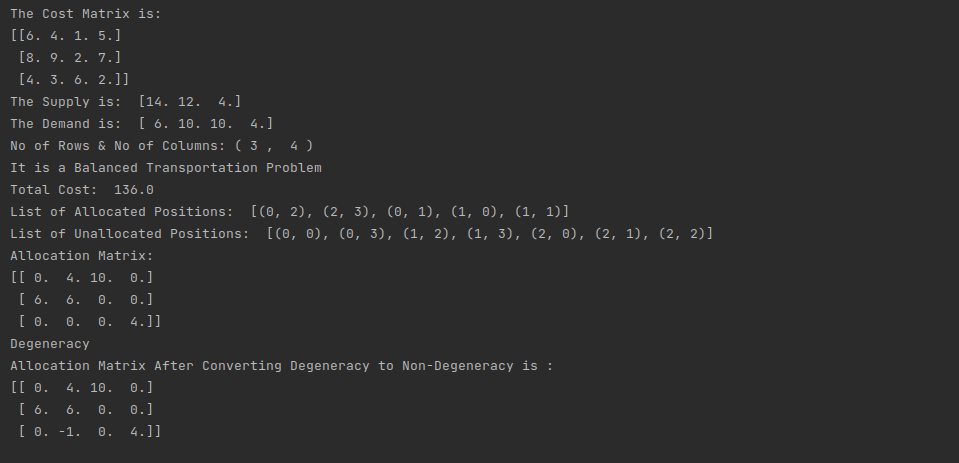
\includegraphics[height=600pt,width=550pt]{Output1}
\pagebreak
\begin{center}
\textbf{\\Problem 2}
\end{center}

\begin{flushleft}
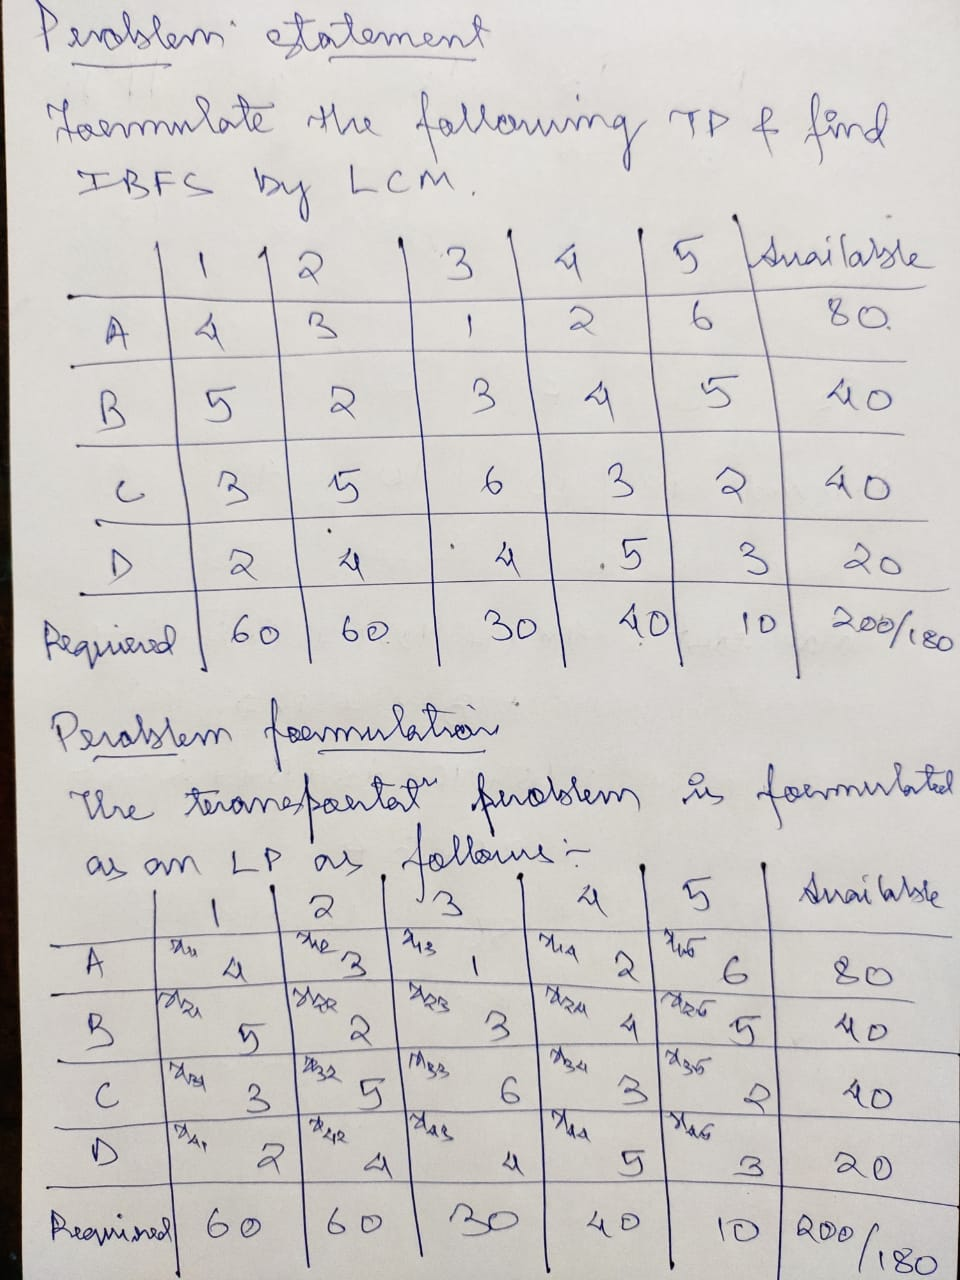
\includegraphics[width=\paperwidth, height=10in]{Page8}
\end{flushleft}
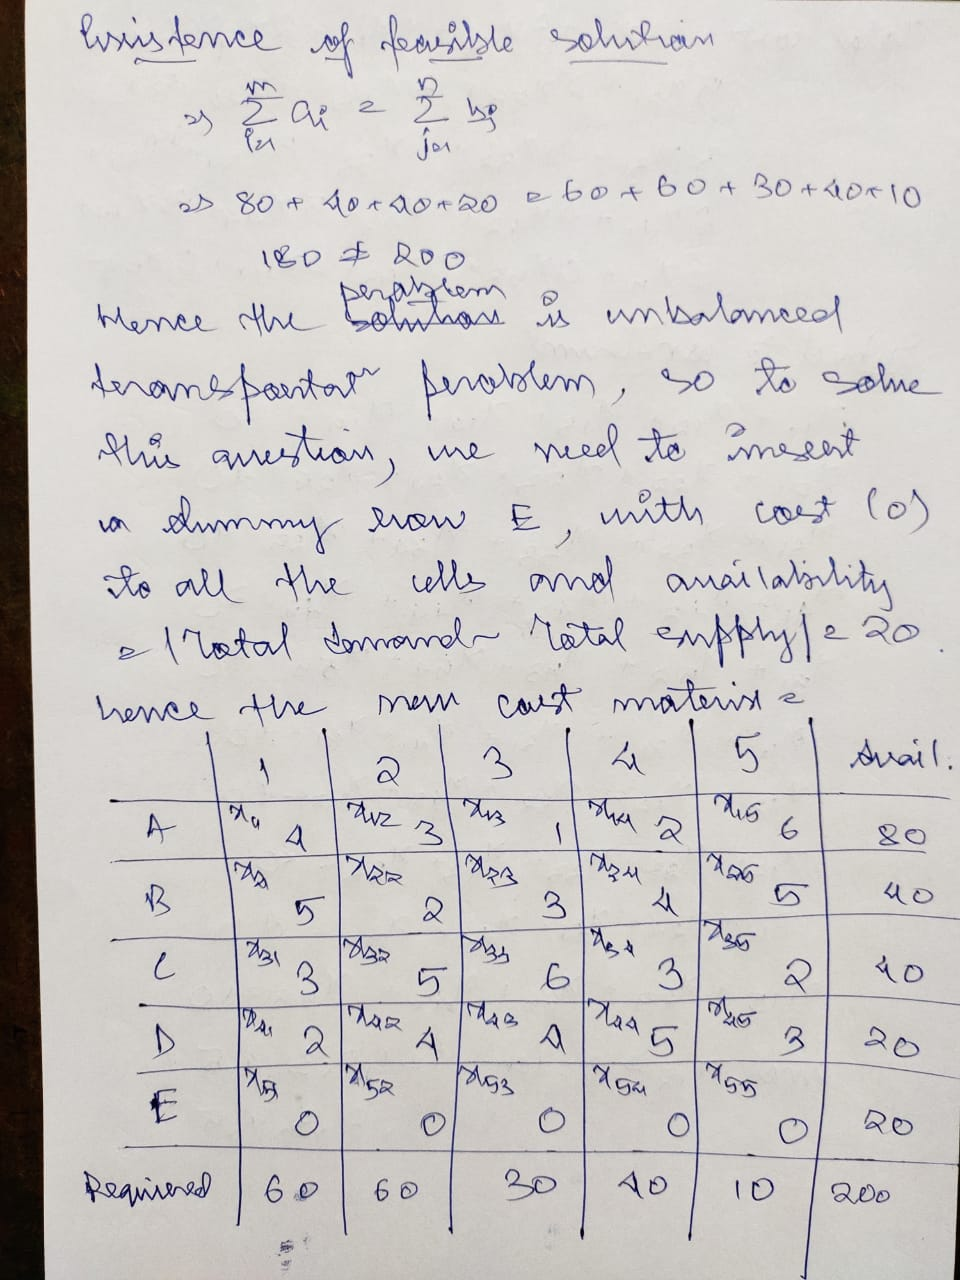
\includegraphics[width=\paperwidth, height=\paperheight]{Page9}
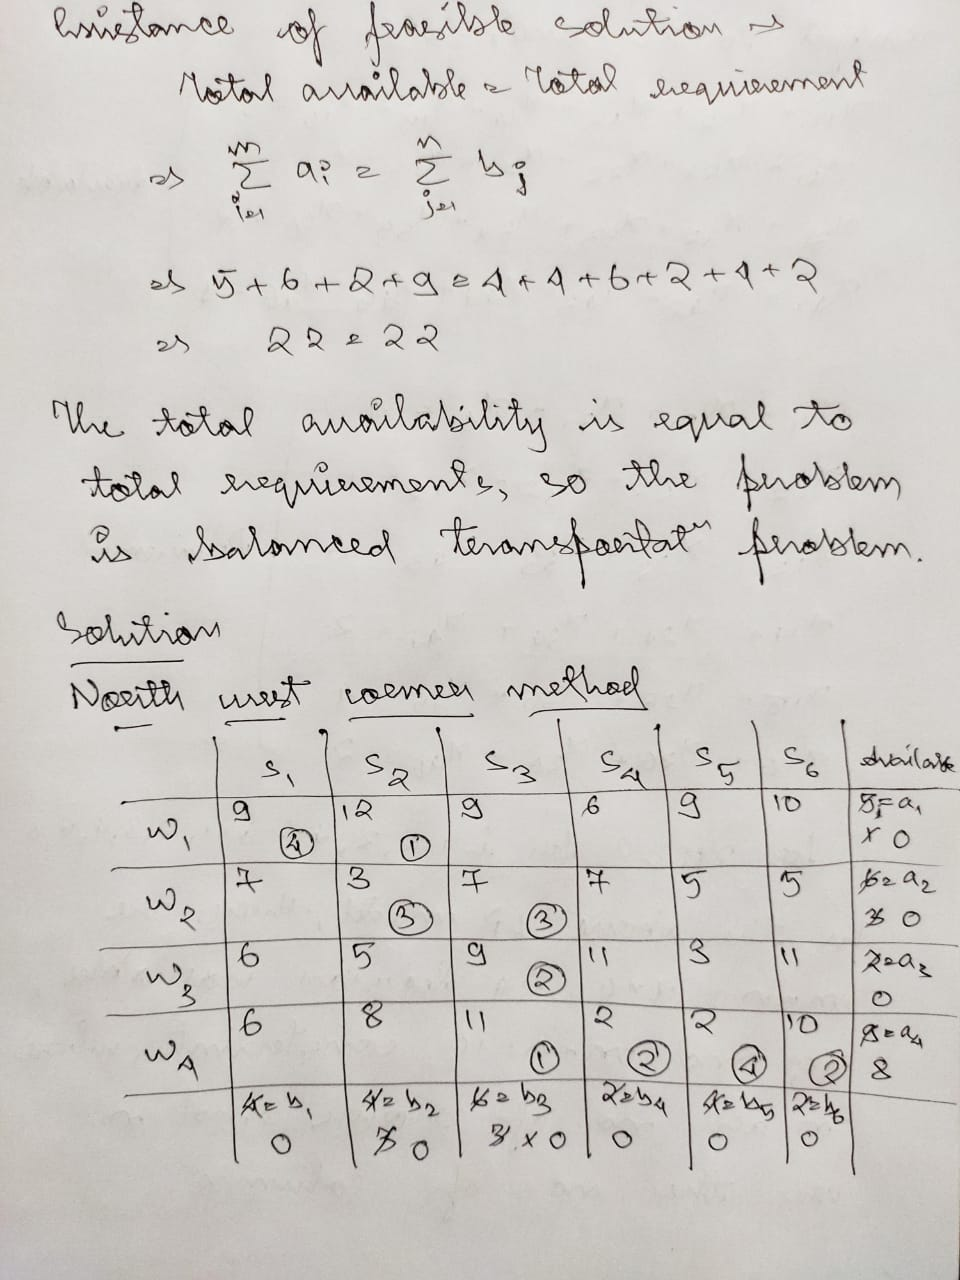
\includegraphics[width=\paperwidth, height=\paperheight]{Page10}
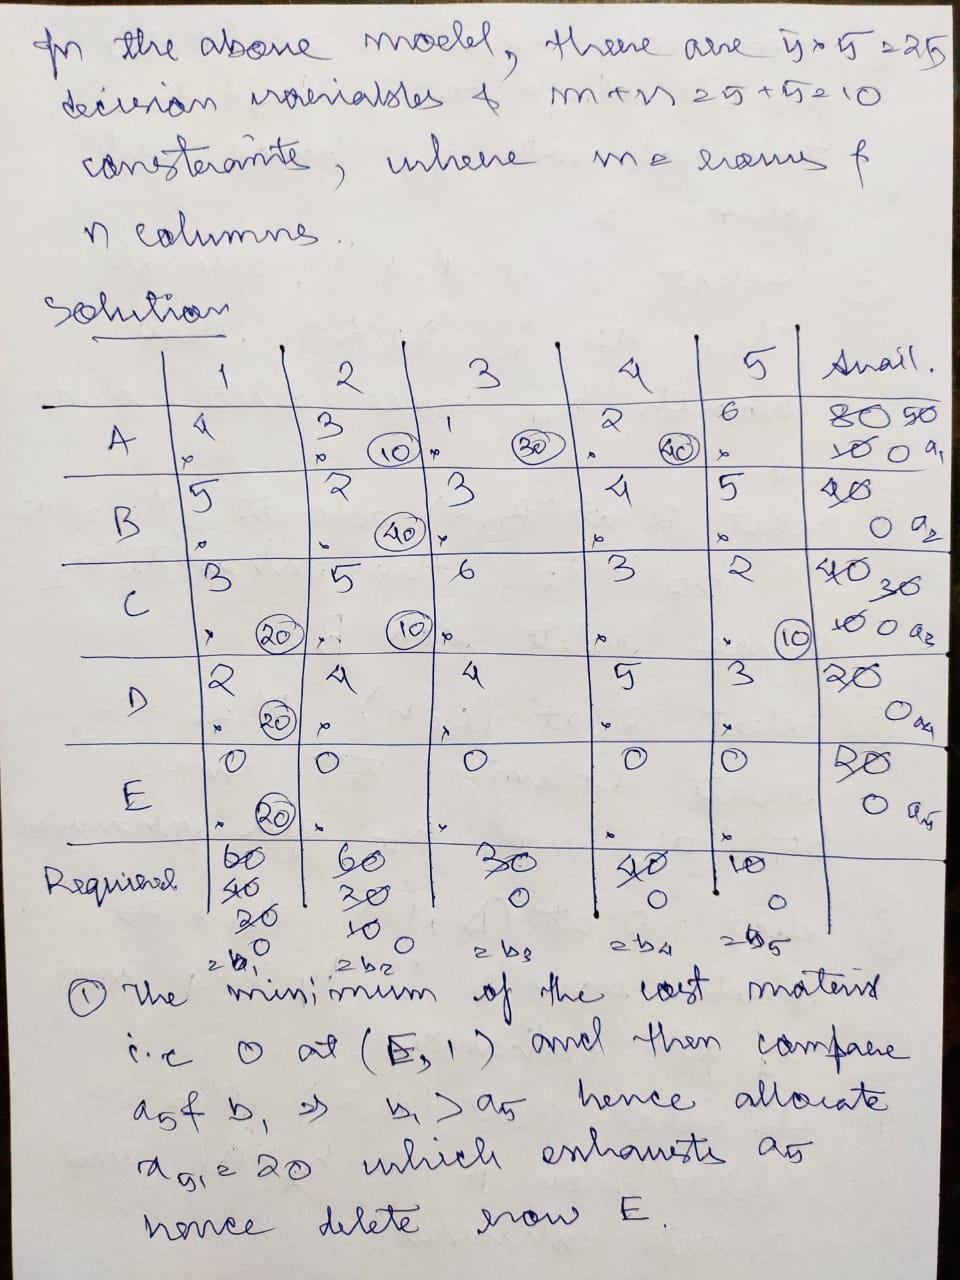
\includegraphics[width=\paperwidth, height=\paperheight]{Page11}
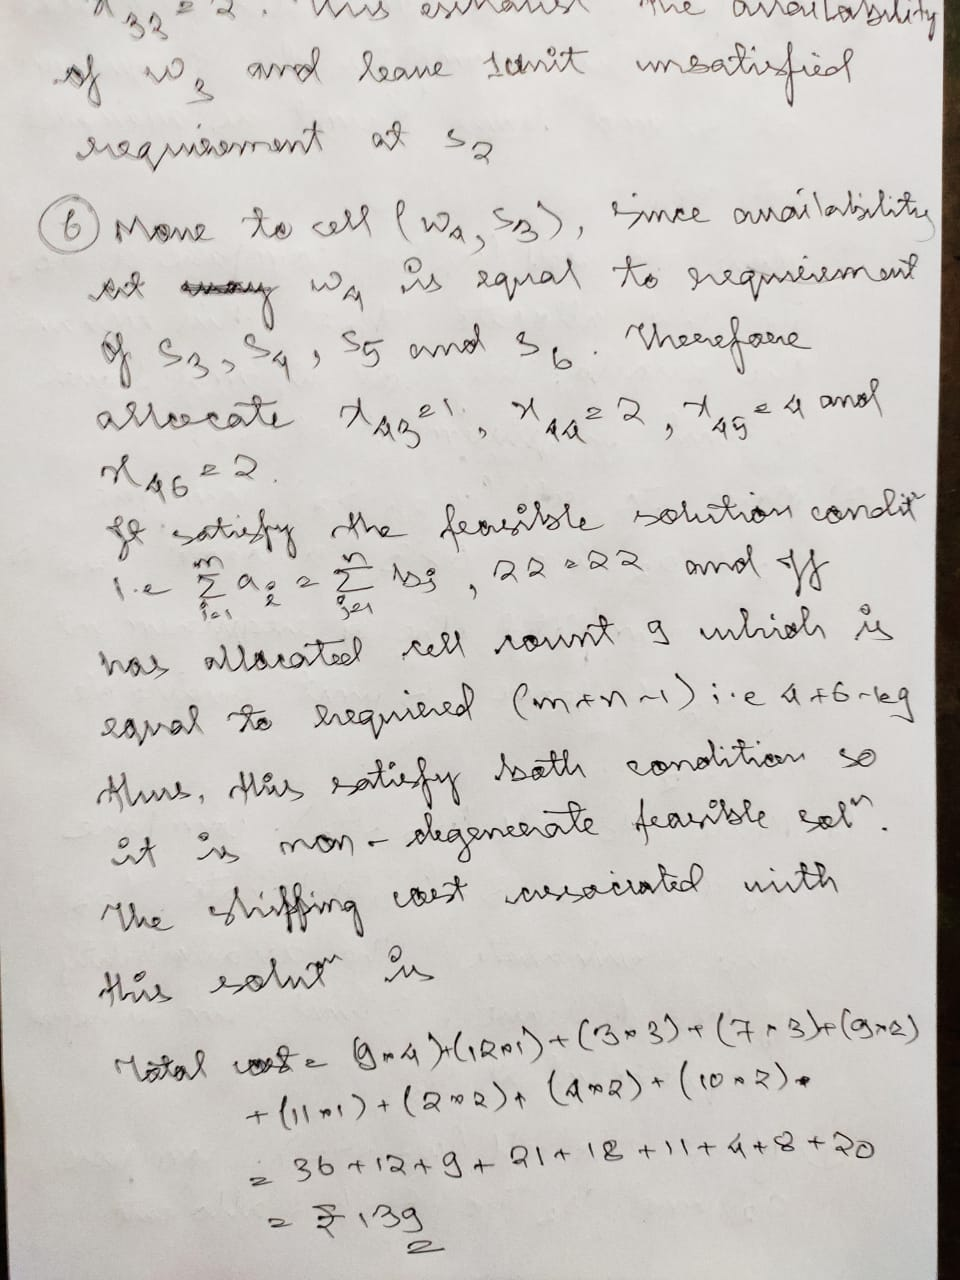
\includegraphics[width=\paperwidth, height=\paperheight]{Page12}
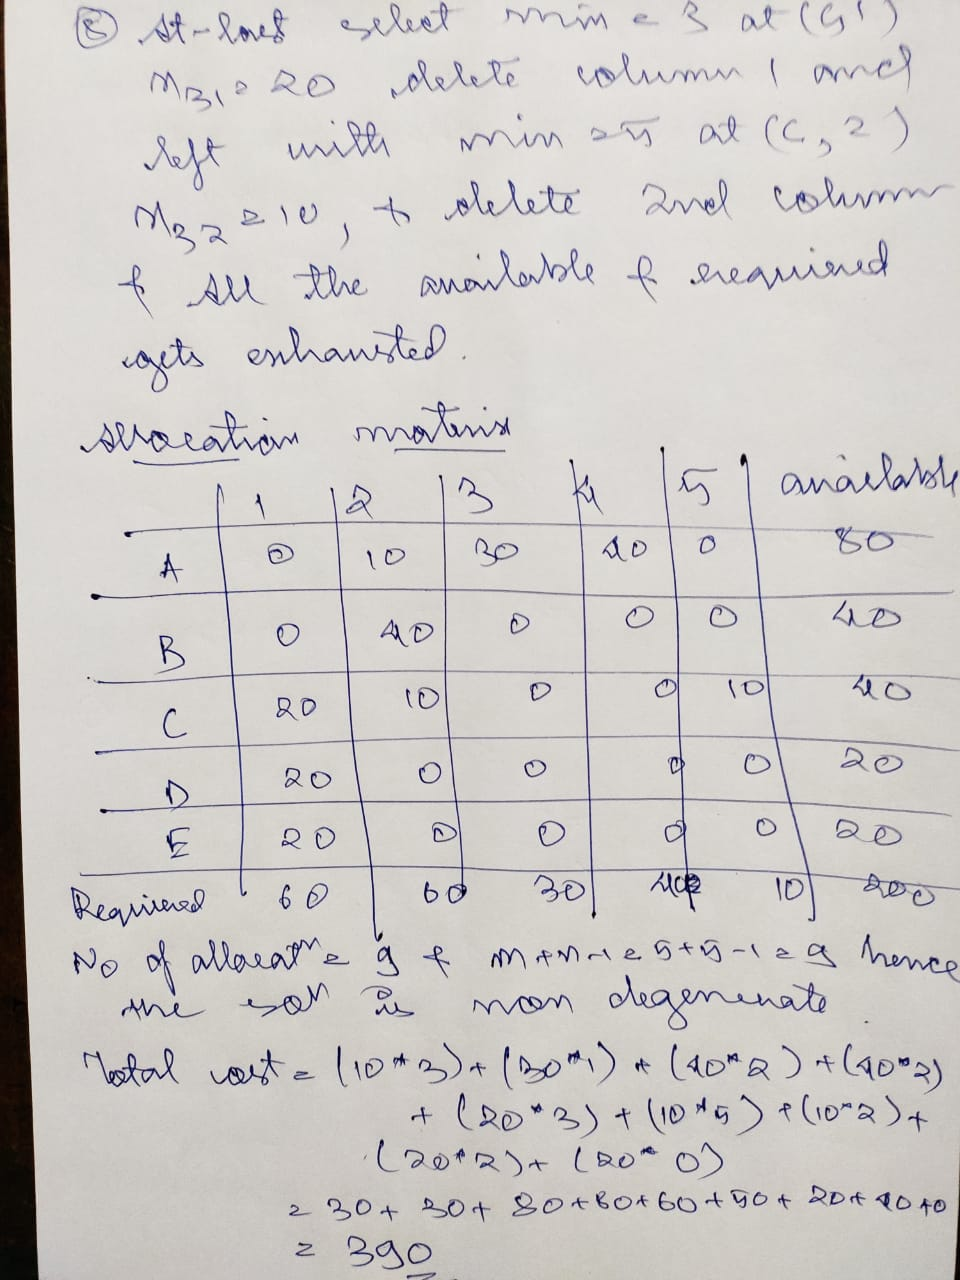
\includegraphics[width=\paperwidth, height=\paperheight]{Page13}
\begin{lstlisting}

	Python Code:
	
	
	import numpy as np
	
	def check_loop(p, row, column):
		p[row, column] = -1
		flag = 1
		while flag != 0:
			flag = 0
			if p.size != 0:
				row = np.count_nonzero(p, axis=1)
				f = 0
				for index in range(len(row)):
					if row[index] < 2:
						flag = 1
						p = np.delete(p, (index - f), axis=0)
						f += 1
			if p.size != 0:
				e = 0
				col = np.count_nonzero(p, axis=0)
				for index in range(len(col)):
					if col[index] < 2:
						flag = 1
						p = np.delete(p, (index - e), axis=1)
						e += 1
		if p.size != 0:
			return 0
		else:
			return 1
		
	if __name__ == '__main__':
		cm = np.array([
			[4.0, 3.0, 1.0, 2.0, 6.0],
			[5.0, 2.0, 3.0, 4.0, 5.0],
			[3.0, 5.0, 6.0, 3.0, 2.0],
			[2.0, 4.0, 4.0, 5.0, 3.0]])
		s = np.array([80.0, 40.0, 40.0, 20.0])
		d = np.array([60.0, 60.0, 30.0, 40.0, 10.0])
		c = cm.copy()
		print("The Cost Matrix is: ")
		print(c)
		print("The Supply is: ", s)
		print("The Demand is: ", d)
		m, n = c.shape
		print("No of Rows & No of Columns: (", m, ", ", n, ")")
		total_cost = 0
		no_alloc = 0
		total_demand = np.sum(d)
		total_supply = np.sum(s)
		alloc = []
		
		
		
		if total_demand == total_supply:
			print("It is a Balanced Transportation Problem")
		else:
			print("It is an UnBalanced Transportation Problem")
			if total_demand > total_supply:
				new = np.array(np.zeros(n))
				c = np.row_stack((c, new))
				s = np.append(s, total_demand - total_supply)
				m = m + 1
			else:
				new = np.array(np.zeros(m))
				c = np.column_stack((c, new))
				d = np.append(d, total_supply - total_demand)
				n = n + 1
			print("The New Balanced Cost Matrix is: ")
			print(c)
			print("The Supply is: ", s)
			print("The Demand is: ", d)
		a = np.zeros(c.shape)
		min_cost = np.amin(c)
		while min_cost != np.inf:
			indexes = np.where(c == min_cost)
			i = indexes[0][0]
			j = indexes[1][0]
			x = min(s[i], d[j])
			s[i] -= x
			d[j] -= x
			total_cost += (x * c[i, j])
			no_alloc += 1
			a[i, j] = x
			alloc.append((i, j))
			if s[i] < d[j]:
				x = 0
				while x < n:
					c[i, x] = np.inf
					x += 1
			elif s[i] > d[j]:
				y = 0
				while y < m:
					c[y, j] = np.inf
					y += 1
			else:
				x = 0
				while x < n:
					c[i, x] = np.inf
					x += 1
				y = 0
				while y < m:
					c[y, j] = np.inf
					y += 1
			min_cost = np.amin(c)
		print("Total Cost: ", total_cost)
		unalloc = []
		
		
		for i in range(m):
			for j in range(n):
				if not (i, j) in alloc:
					unalloc.append((i, j))
		print("List of Allocated Positions: ", alloc)
		print("List of Unallocated Positions: ", unalloc)
		print("Allocation Matrix: ")
		print(a)
		no_loop = []
		if no_alloc == m + n - 1:
			print("Non Degeneracy")
		else:
			print("Degeneracy")
			for i in unalloc:
				g = check_loop(a.copy(), i[0], i[1])
				if g == 1:
					no_loop.append(i)
			min_epi_list = []
			for i in no_loop:
				min_epi_list.append(cm[i[0], i[1]])
			min_epi = min(min_epi_list)
			ind = min_epi_list.index(min_epi)
			loc = no_loop[ind]
			a[loc[0], loc[1]] = -1
			print("Allocation Matrix After Converting 
				Degeneracy to Non-Degeneracy is : ")
			print(a)

\end{lstlisting}
\pagebreak
\begin{lstlisting}
	
	Output:
	
\end{lstlisting}

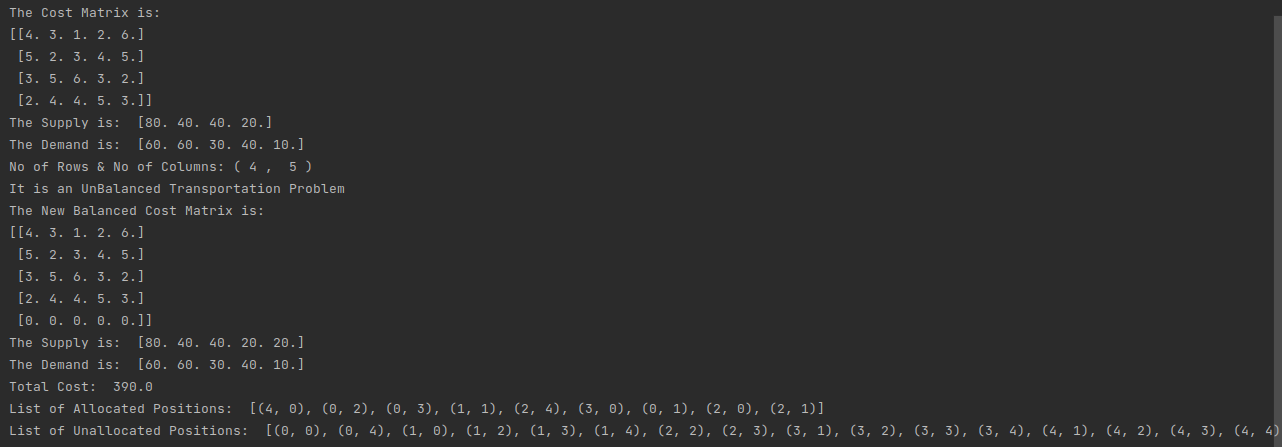
\includegraphics[height=300pt,width=550pt]{Output2}


\includegraphics[height=200pt,width=550pt]{Output3}

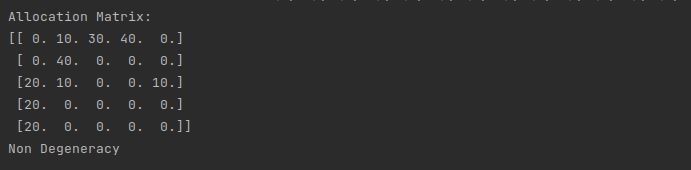
\includegraphics[height=200pt,width=550pt]{Output4}
\end{document}
